\documentclass[11pt]{article}

\usepackage[english]{babel}
\usepackage[utf8]{inputenc}
\usepackage[T1]{fontenc}
\usepackage[margin=1in]{geometry}
\usepackage{amsmath, amssymb, amsfonts, amsthm, mathtools}
\usepackage{physics}
\usepackage{graphicx}
\usepackage{booktabs}
\usepackage{enumitem}
\usepackage{fancyhdr}
\usepackage[most]{tcolorbox}
\usepackage[colorlinks=true, allcolors=blue]{hyperref}

\graphicspath{{figures/}}
\setlength{\emergencystretch}{3em}
\numberwithin{equation}{section}

\providecommand{\erf}{\operatorname{erf}}
\providecommand{\erfc}{\operatorname{erfc}}
\newcommand{\lth}{\lambda_{\mathrm{th}}}
\newcommand{\Cq}{C_v^{\mathrm{q}}}
\newcommand{\Ccl}{C_v^{\mathrm{cl}}}
\newcommand{\kB}{k_{B}}
\newcommand{\Eu}{\hbar^2\alpha^2/2m}

\newtcolorbox{resultbox}[1]{
    colback=lightgray!15, colframe=black, arc=3pt, outer arc=3pt,
    boxrule=0.8pt, left=2mm, right=2mm, top=2mm, bottom=2mm, breakable,
    title={#1}, colbacktitle=gray!20, coltitle=black, fonttitle=\bfseries
}
\newtcolorbox{checkbox}{
    colback=white, colframe=gray!60, arc=2pt, boxrule=0.5pt,
    left=2mm, right=2mm, top=1mm, bottom=1mm, breakable
}

\pagestyle{fancy}
\fancyhf{}
\lhead{\small 00540367: Research Project 1}
\rhead{\small Technion - IIT}
\lfoot{\small Spring 2026 | Semester 6}
\rfoot{\small Page \thepage}
\renewcommand{\headrulewidth}{0.4pt}
\renewcommand{\footrulewidth}{0.4pt}

\title{P\"oschl--Teller Well in a Box:\\Full Derivations Behind the Summary}
\author{Nadav Jean\\[1mm]
\small Department of Chemical Engineering, Technion -- Israel Institute of Technology}
\date{\small For my own verification before the meeting of 28.10.2026}

\begin{document}
\maketitle
\thispagestyle{fancy}

\begin{resultbox}{How to use this document}
Each section derives one part of \texttt{PT\_Box\_Summary.pdf}, in the same order:
\begin{center}
\begin{tabular}{lll}
\toprule
Summary & What & Here\\
\midrule
Sec.~1, Eq.~(1) & potential, source of its form & Sec.~\ref{sec:model}\\
Sec.~2, Eq.~(2) & energy levels & Sec.~\ref{sec:levels}\\
Sec.~3, Eqs.~(3)--(4) & $Z_q$ and $\Cq$ & Sec.~\ref{sec:quantum}\\
Sec.~4, Eqs.~(5)--(6) & $Z_{\rm cl}$ and $\Ccl$ & Sec.~\ref{sec:classical}\\
Sec.~5, ``box alone'' & empty-box excess, $\le\kB/16$ & Sec.~\ref{sec:box}\\
Sec.~5, mechanism and numbers & desorption picture, anomaly table & Sec.~\ref{sec:mechanism}\\
Sec.~6 & homogeneous strokes, $W=(q-1)\int C_v\,\dd T$ & Sec.~\ref{sec:stroke}\\
\bottomrule
\end{tabular}
\end{center}
Every number is reproduced by \texttt{check\_formulas.py} (about 10~s) and every figure by \texttt{make\_figures.py}, both in this folder. The boxes marked \textbf{Check} list what each step relies on, so it can be verified line by line. Sec.~\ref{sec:verify} lists the references whose exact section or problem numbers should be confirmed in a library copy before quoting them.
\end{resultbox}

\tableofcontents

% =====================================================================
\section{The model and its two dimensionless numbers}
\label{sec:model}
A particle of mass $m$ moves in one dimension with $H=p^2/2m+V(x)$, where
\begin{equation}
V(x)=\begin{cases}
-\dfrac{\hbar^2}{2m}\,\alpha^2\,\dfrac{\lambda(\lambda-1)}{\cosh^2(\alpha x)}, & |x|<L/2,\\[6pt]
+\infty, & |x|\ge L/2.
\end{cases}
\label{eq:Vgeneral}
\end{equation}
Inside the box this is the ``modified P\"oschl--Teller well'' written exactly as in Table~I of Deffner, Jarzynski and del Campo~\cite{deffner2014} (their $q$ is our $x$). The table takes it from Fl\"ugge~\cite{flugge}, and the original is Ref.~\cite{poschlteller}. We take $\lambda=2$, so $\lambda(\lambda-1)=2$ and
\begin{equation}
V(x)=-\frac{\hbar^2}{2m}\,\alpha^2\,\frac{2}{\cosh^2(\alpha x)}=-\frac{\hbar^2\alpha^2}{m}\,\frac{1}{\cosh^2(\alpha x)}\qquad(|x|<L/2).
\label{eq:V2}
\end{equation}
The well has depth $\hbar^2\alpha^2/m$ (classical floor $V_{\min}=-\hbar^2\alpha^2/m$ at $x=0$) and width $\sim1/\alpha$. For integer $\lambda$ the well is \emph{reflectionless}: Landau and Lifshitz~\cite{LL} give the transmission coefficient of $U_0/\cosh^2(\alpha x)$, and for the attractive case with $U_0=-\frac{\hbar^2\alpha^2}{2m}\lambda(\lambda-1)$ it equals 1 at every energy when $\lambda$ is an integer (see also Refs.~\cite{lekner,CKS}). This is what makes the spectrum below exact.

\paragraph{Helpers.} Only these derivation-local combinations are used, each defined in physical constants:
\begin{equation}
a\equiv\frac{\beta\hbar^2\alpha^2}{m}=\frac{\text{well depth}}{\kB T},\qquad
\lth\equiv\sqrt{\frac{2\pi\hbar^2\beta}{m}},\qquad
\frac{L}{\lth}=\frac{\alpha L}{\sqrt{2\pi a}},\qquad
\frac{\kB T}{\Eu}=\frac{2}{a}.
\label{eq:helpers}
\end{equation}
The last two identities follow from $\lth^2=2\pi\hbar^2\beta/m=2\pi a/\alpha^2$. Every result below depends on $\alpha L$ and $a$ only, i.e.\ on $\alpha L$ and $\kB T/(\Eu)$. Temperatures are quoted as $\kB T$ in units of $\Eu$.

\paragraph{The wall region.} At the wall, $|V(\pm L/2)|=(\hbar^2\alpha^2/m)/\cosh^2(\alpha L/2)\approx4(\hbar^2\alpha^2/m)\,e^{-\alpha L}$. Every approximation below drops terms of this order, which is below $10^{-40}$ of the depth for the cases used ($\alpha L\ge100$).

% =====================================================================
\section{Energy levels}
\label{sec:levels}

\subsection{Factorization: the well is the partner of the free particle}
Following the supersymmetric method of Cooper, Khare and Sukhatme~\cite{CKS}, define the superpotential $W(x)=\frac{\hbar\alpha}{\sqrt{2m}}\tanh(\alpha x)$ and
\begin{equation}
A=\frac{\hbar}{\sqrt{2m}}\dv{x}+W(x),\qquad A^\dagger=-\frac{\hbar}{\sqrt{2m}}\dv{x}+W(x).
\end{equation}
Acting on a test function $f$, $A^\dagger Af=-\frac{\hbar^2}{2m}f''+\big(W^2-\frac{\hbar}{\sqrt{2m}}W'\big)f$ and $AA^\dagger f=-\frac{\hbar^2}{2m}f''+\big(W^2+\frac{\hbar}{\sqrt{2m}}W'\big)f$. With $W^2=\frac{\hbar^2\alpha^2}{2m}\tanh^2(\alpha x)$, $\frac{\hbar}{\sqrt{2m}}W'=\frac{\hbar^2\alpha^2}{2m}\frac{1}{\cosh^2(\alpha x)}$ and $\tanh^2=1-1/\cosh^2$:
\begin{align}
A^\dagger A&=-\frac{\hbar^2}{2m}\dv[2]{x}-\frac{\hbar^2\alpha^2}{m}\,\frac{1}{\cosh^2(\alpha x)}+\frac{\hbar^2\alpha^2}{2m}=H_{\rm PT}+\frac{\hbar^2\alpha^2}{2m},\\
AA^\dagger&=-\frac{\hbar^2}{2m}\dv[2]{x}+\frac{\hbar^2\alpha^2}{2m}=H_{0}+\frac{\hbar^2\alpha^2}{2m},
\end{align}
where $H_{\rm PT}$ has the potential of Eq.~\eqref{eq:V2} and $H_0$ is the free particle. Multiplying $AA^\dagger=H_0+\hbar^2\alpha^2/2m$ on the left by $A^\dagger$ and using the first line gives the intertwining relation $H_{\rm PT}A^\dagger=A^\dagger H_0$. So if $H_0\phi=E\phi$ then $H_{\rm PT}(A^\dagger\phi)=E(A^\dagger\phi)$. With $\phi=e^{ikx}$, $E=\hbar^2k^2/2m$, and dropping a constant factor,
\begin{equation}
\boxed{\;\psi_k(x)=\big(\alpha\tanh(\alpha x)-ik\big)\,e^{ikx},\qquad E=\frac{\hbar^2k^2}{2m}.\;}
\label{eq:jost}
\end{equation}
This solves the Schr\"odinger equation inside the box for every $k$, real or complex; no boundary condition has been used yet. Appendix~\ref{app:check} checks it by direct differentiation, and Lekner~\cite{lekner} gives the same solutions.

\begin{checkbox}
\textbf{Check.} (i) $\dv{x}\tanh(\alpha x)=\alpha/\cosh^2(\alpha x)$. (ii) Appendix~\ref{app:check}. (iii) Reflectionless: as $x\to\pm\infty$, $\psi_k\to(\pm\alpha-ik)e^{ikx}$, a pure right-moving wave on both sides, with no $e^{-ikx}$ (reflected) part.
\end{checkbox}

\subsection{Solutions of definite parity}
$V$ is even, so the eigenstates have definite parity. For real $k$, the real and imaginary parts of Eq.~\eqref{eq:jost} supply both:
\begin{align}
\psi_o(x)&=\mathrm{Re}\,\psi_k=\alpha\tanh(\alpha x)\cos(kx)+k\sin(kx) &&\text{(odd)},\label{eq:psio}\\
\psi_e(x)&=-\mathrm{Im}\,\psi_k=k\cos(kx)-\alpha\tanh(\alpha x)\sin(kx) &&\text{(even)}.\label{eq:psie}
\end{align}

\subsection{Box levels (\texorpdfstring{$E>0$}{E > 0})}
By parity, $\psi(\pm L/2)=0$ reduces to one condition at $x=L/2$, where $\alpha\tanh(\alpha x)=\alpha\tanh(\alpha L/2)\equiv c$ (a derivation-local constant, $c=\alpha[1+\mathcal O(e^{-\alpha L})]$):
\begin{align}
\text{even:}\quad& k\cos(kL/2)=c\,\sin(kL/2)\iff \tan(kL/2)=k/c,\\
\text{odd:}\quad& c\cos(kL/2)+k\sin(kL/2)=0\iff \tan(kL/2)=-c/k .
\end{align}
Let $\varphi(k)=\arctan(k/c)\in(0,\pi/2)$. The even condition is $kL/2=\varphi+\ell\pi$. Since $-c/k=-\cot\varphi=\tan(\varphi+\pi/2)$, the odd condition is $kL/2=\varphi+\pi/2+\ell\pi$. Together:
\begin{equation}
\boxed{\;k_jL=j\pi+2\arctan\!\left(\frac{k_j}{\alpha\tanh(\alpha L/2)}\right),\qquad E_j=\frac{\hbar^2k_j^2}{2m},\qquad j=1,2,3,\dots\;}
\label{eq:quant}
\end{equation}
with even $j$ for even states and odd $j$ for odd states. Dropping $\mathcal O(e^{-\alpha L})$, $\alpha\tanh(\alpha L/2)\to\alpha$, which is Eq.~(2) of the summary.

\paragraph{Exactly one root per $j$.} Let $f(k)=kL-2\arctan(k/c)$. Then $f(0)=0$ and $f'(k)=L-2c/(k^2+c^2)\ge L-2/c>0$ whenever $cL>2$ (i.e.\ $\alpha L\gtrsim2.4$). So $f$ is increasing and each $j\ge1$ has one root, in the bracket $j\pi/L<k_j<(j+1)\pi/L$ because $0<2\arctan<\pi$. The value $j=0$ gives only $k=0$, where $\psi_e\equiv0$ and $\psi_o=\alpha\tanh(\alpha x)$ does not vanish at the wall, so it is not a state.

\paragraph{Solving it.} The fixed-point iteration $k\leftarrow[j\pi+2\arctan(k/c)]/L$, started at $k=j\pi/L$, contracts by a factor $\le2/(cL)$ per step (0.1 at $\alpha L=20$). \texttt{check\_formulas.py} reaches residuals of $10^{-15}$.

\subsection{The bound state (\texorpdfstring{$E<0$}{E < 0})}
Set $k=i\kappa$, $\kappa>0$, so $E=-\hbar^2\kappa^2/2m$. With $\cos(i\kappa x)=\cosh\kappa x$ and $\sin(i\kappa x)=i\sinh\kappa x$, Eqs.~\eqref{eq:psio}--\eqref{eq:psie} give the real solutions
\begin{equation}
\chi_e=\kappa\cosh(\kappa x)-\alpha\tanh(\alpha x)\sinh(\kappa x),\qquad
\chi_o=\alpha\tanh(\alpha x)\cosh(\kappa x)-\kappa\sinh(\kappa x).
\end{equation}
\begin{itemize}[itemsep=2pt]
\item \textbf{Even:} $\chi_e(L/2)=0\iff$
\begin{equation}
\boxed{\;\kappa_b=\alpha\tanh(\alpha L/2)\tanh(\kappa_bL/2),\qquad E_b=-\frac{\hbar^2\kappa_b^2}{2m}=-\frac{\hbar^2\alpha^2}{2m}\left[1-8e^{-\alpha L}+\dots\right].\;}
\label{eq:bound}
\end{equation}
$g(\kappa)=c\tanh(\kappa L/2)-\kappa$ has $g(0)=0$, $g'(0)=cL/2-1>0$ and is concave, so there is exactly one root, with $\kappa_b<c<\alpha$. At $\alpha L=20$, $E_b/(\Eu)=-0.99999998351$, matching $1-8e^{-20}$. The wavefunction is $\chi_e\to\alpha/\cosh(\alpha x)$ as $\kappa\to\alpha$ (use $\cosh(\alpha x)-\tanh(\alpha x)\sinh(\alpha x)=1/\cosh(\alpha x)$).
\item \textbf{Odd:} $\chi_o(L/2)=0\iff\kappa\tanh(\kappa L/2)=c$, whose only root is $\kappa=\alpha$ up to $e^{-\alpha L}$. But there $\chi_o\equiv0$, because $\alpha\tanh(\alpha x)\cosh(\alpha x)=\alpha\sinh(\alpha x)$, so the root is spurious. At $E=-\hbar^2\alpha^2/2m$ the second (odd) solution is $[x/2+\sinh(2\alpha x)/4\alpha]/\cosh(\alpha x)$, positive for all $x>0$, so it cannot vanish at the wall. Hence there is \emph{no odd bound state}.
\end{itemize}

\begin{checkbox}
\textbf{Check against the textbook.} Landau and Lifshitz~\cite{LL} give the bound levels of $-U_0/\cosh^2(\alpha x)$ on the open line:
$E_n=-\frac{\hbar^2\alpha^2}{8m}\big[-(1+2n)+\sqrt{1+8mU_0/\alpha^2\hbar^2}\big]^2$, $n=0,1,\dots$ while the bracket is positive. With $U_0=\frac{\hbar^2\alpha^2}{2m}\lambda(\lambda-1)$, $\sqrt{1+4\lambda(\lambda-1)}=2\lambda-1$, so $E_n=-\frac{\hbar^2\alpha^2}{2m}(\lambda-1-n)^2$ for $n<\lambda-1$. For $\lambda=2$: one level, $n=0$, $E_0=-\hbar^2\alpha^2/2m$. This agrees with Eq.~\eqref{eq:bound} as $\alpha L\to\infty$.
\end{checkbox}

\subsection{Physical reading: phase shift and Levinson's theorem}
For the empty box $k_jL=j\pi$. The well adds $2\arctan(k/\alpha)\in(0,\pi)$, so every box level is pushed up, by less than one spacing (Table~\ref{tab:levels}). As $k\to\infty$ the addition tends to $\pi$, so level $j$ approaches level $j+1$ of the empty box: one state has left the continuum, and it reappears as the bound state.

In the standard convention the scattering phase shift is $\delta(k)=\pi-2\arctan(k/\alpha)=2\arctan(\alpha/k)$, and Eq.~\eqref{eq:quant} reads $k_jL=(j+1)\pi-\delta(k_j)$. It falls from $\delta(0)=\pi$ to $\delta(\infty)=0$, and $\delta(0)-\delta(\infty)=\pi\times(\text{one bound state})$ is Levinson's theorem~\cite{levinson}. The counting above shows the same thing directly from the bracket $j\pi/L<k_j<(j+1)\pi/L$. The level density used in Sec.~\ref{sec:quantum} is $\dd j/\dd k=[L+\dd\delta/\dd k]/\pi$.

\begin{table}[h]
\centering
\caption{The levels drawn in the summary's Fig.~1(a), $\alpha L=20$, in units of $\Eu$ (\texttt{check\_formulas.py}, section 1).}
\label{tab:levels}
\begin{tabular}{cccccc}
\toprule
 & bound & $j=1$ & $j=2$ & $j=3$ & $j=4$\\
\midrule
PT + box, Eqs.~\eqref{eq:quant}--\eqref{eq:bound} & $-0.99999998$ & 0.030394 & 0.120836 & 0.269487 & 0.474202\\
empty box, $(j\pi/\alpha L)^2$ & -- & 0.024674 & 0.098696 & 0.222066 & 0.394784\\
\bottomrule
\end{tabular}
\end{table}

% =====================================================================
\section{Quantum partition function and heat capacity}
\label{sec:quantum}

\subsection{The variance formula}
For levels $\{E_n\}$, $Z=\sum_ne^{-\beta E_n}$, $\expval{E}=-\partial_\beta\ln Z$ and $\expval{E^2}=Z^{-1}\partial_\beta^2Z$. With $\partial_T=-\kB\beta^2\partial_\beta$,
\begin{equation}
C_v=\pdv{\expval{E}}{T}=\kB\beta^2\,\pdv[2]{\ln Z}{\beta}=\kB\beta^2\left(\expval{E^2}-\expval{E}^2\right)=\kB\beta^2\,\mathrm{Var}(E),
\label{eq:var}
\end{equation}
the standard energy-fluctuation result of the canonical ensemble (Pathria and Beale~\cite{pathria}, \S3.6). Since $a=\beta\hbar^2\alpha^2/m$ is proportional to $\beta$, $\beta\,\partial_\beta=a\,\partial_a$ and $\beta^2\partial_\beta^2=a^2\partial_a^2$, so equivalently $C_v=\kB\,a^2\,\partial_a^2\ln Z$. Here
\begin{equation}
Z_q=e^{-\beta E_b}+\sum_{j=1}^{\infty}e^{-\beta E_j}.
\label{eq:Zqsum}
\end{equation}

\subsection{The sum over box levels by Poisson summation}
\label{sec:poisson}
Let $j(k)=[kL-2\arctan(k/c)]/\pi$ be the counting function implied by Eq.~\eqref{eq:quant}, $k(j)$ its inverse, and $F(j)=\exp[-\beta\hbar^2k(j)^2/2m]$, so the box sum is $\sum_{j\ge1}F(j)$. Since $\arctan$ is odd, $j(k)$ and $k(j)$ are odd, so $F$ is even with $F(0)=1$. The Poisson summation formula (DLMF \S1.8(iv)~\cite{dlmf}), $\sum_{j\in\mathbb Z}F(j)=\sum_{\ell\in\mathbb Z}\hat F(\ell)$ with $\hat F(\ell)=\int F(y)e^{-2\pi i\ell y}\dd y$, applied to an even $F$ gives $2\sum_{j\ge1}F(j)+F(0)=\hat F(0)+2\sum_{\ell\ge1}\hat F(\ell)$, i.e.
\begin{equation}
\sum_{j=1}^{\infty}F(j)=\int_0^\infty F(j)\,\dd j-\frac12+R,\qquad R=\sum_{\ell\ge1}\hat F(\ell).
\label{eq:poisson}
\end{equation}
$R$ is exponentially small. For the empty box, $\hat F(\ell)=(2L/\lth)\,e^{-4\pi\ell^2(L/\lth)^2}$ (a Gaussian's Fourier transform), and the well only adds terms small in $e^{-\alpha L}$. It is below double precision whenever $L\gtrsim\lth$ (Sec.~\ref{sec:box} shows where it starts to matter).

\subsection{The integral, using the level density}
Change variables from $j$ to $k$. The level density, read off Eq.~\eqref{eq:quant}, is
\begin{equation}
\dv{j}{k}=\frac1\pi\left[L-\frac{2c}{k^2+c^2}\right].
\end{equation}
The first term is the empty box; the second, $\frac1\pi\dv{k}[2\arctan(k/c)]$, is the change in the density of states caused by the phase shift, which is the Beth--Uhlenbeck idea~\cite{BU,DMB}. With the derivation-local $b=\beta\hbar^2/2m$ (so $\lth=\sqrt{4\pi b}$):
\begin{align}
\int_0^\infty F\,\dd j&=\frac{L}{\pi}\int_0^\infty e^{-bk^2}\dd k-\frac{2c}{\pi}\int_0^\infty\frac{e^{-bk^2}}{k^2+c^2}\,\dd k\nonumber\\
&=\frac{L}{\pi}\cdot\frac12\sqrt{\frac{\pi}{b}}-\frac{2c}{\pi}\cdot\frac{\pi}{2c}\,e^{bc^2}\erfc\!\big(c\sqrt b\big)
=\frac{L}{\lth}-e^{bc^2}\erfc\!\big(c\sqrt b\big).
\end{align}
The second integral is Gradshteyn--Ryzhik 3.466.1~\cite{GR}, derived in Appendix~\ref{app:gaussint}.

\subsection{The closed form}
Add the bound state, $e^{-\beta E_b}=e^{\beta\hbar^2\kappa_b^2/2m}$:
\begin{equation}
Z_q=\frac{L}{\lth}-\frac12+e^{\beta\hbar^2\kappa_b^2/2m}-e^{bc^2}\erfc\big(c\sqrt b\big)+R .
\end{equation}
Both $\kappa_b$ and $c$ equal $\alpha[1+\mathcal O(e^{-\alpha L})]$, and $b\alpha^2=\beta\hbar^2\alpha^2/2m=a/2$. Using $1-\erfc=\erf$:
\begin{equation}
\boxed{\;Z_q=\frac{L}{\lth}-\frac12+e^{a/2}\erf\sqrt{a/2}\,,\qquad a=\frac{\beta\hbar^2\alpha^2}{m}.\;}
\label{eq:Zq}
\end{equation}
\textbf{Reading.} $L/\lth$: free particle in the box. $-\tfrac12$: hard-wall (Dirichlet) correction, half a state missing. $e^{a/2}=e^{-\beta E_b}$: the bound state. $-e^{a/2}\erfc\sqrt{a/2}$: the continuum state that became the bound state, removed with the energy spread set by the phase shift. The Beth--Uhlenbeck form of this result is $Z=Z_{\rm free}+\sum_be^{-\beta E_b}+\frac1\pi\int\dv{\delta}{k}e^{-\beta\hbar^2k^2/2m}\dd k$~\cite{BU}, which is what the two lines above evaluate.

\begin{checkbox}
\textbf{Check.} (i) $\frac{L}{\pi}\cdot\frac12\sqrt{\pi/b}=L/\sqrt{4\pi b}=L/\lth$. (ii) Appendix~\ref{app:gaussint}. (iii) Numerically, Eq.~\eqref{eq:Zq} with Eq.~\eqref{eq:Cq} below against $\mathrm{Var}(E)$ over the exact levels of Eqs.~\eqref{eq:quant}--\eqref{eq:bound}: max difference $1.1\times10^{-13}\kB$, $2.2\times10^{-13}\kB$ and $2.1\times10^{-13}\kB$ for $\alpha L=60$, $100$ and $1000$, over $\kB T\in[0.02,5]\,(\Eu)$, using 381, 602 and 5564 levels.
\end{checkbox}

\subsection{Closed-form \texorpdfstring{$\Cq$}{Cq}}
Write $Z_q=B(a)-\frac12+G(a)$ with $B=L/\lth=\alpha L/\sqrt{2\pi a}$ and $G=e^{a/2}\erf\sqrt{a/2}$. Primes are $\dd/\dd a$. Since $B\propto a^{-1/2}$,
\begin{equation}
B'=-\frac{B}{2a},\qquad B''=\frac{3B}{4a^2}.
\end{equation}
From $\erf z=\frac{2}{\sqrt\pi}\int_0^ze^{-s^2}\dd s$~\cite{dlmf}, $\dv{a}\erf\sqrt{a/2}=\frac{2}{\sqrt\pi}e^{-a/2}\cdot\frac{1}{2\sqrt{2a}}=\frac{e^{-a/2}}{\sqrt{2\pi a}}$, so
\begin{equation}
G'=\frac12G+\frac{1}{\sqrt{2\pi a}},\qquad G''=\frac12G'-\frac{1}{2\sqrt{2\pi}}\,a^{-3/2}.
\end{equation}
Then $Z_q'=B'+G'$, $Z_q''=B''+G''$, and Eq.~\eqref{eq:var} becomes
\begin{equation}
\boxed{\;\frac{\Cq}{\kB}=a^2\left[\frac{Z_q''}{Z_q}-\left(\frac{Z_q'}{Z_q}\right)^2\right].\;}
\label{eq:Cq}
\end{equation}
(In \texttt{cv\_plot.py}, $Z_q$, $Z_q'$ and $Z_q''$ are all multiplied by $e^{-a/2}$ before dividing. The ratios are unchanged and nothing overflows at low $T$.)

\subsection{Limits}
\label{sec:Cqlimits}
\begin{itemize}[itemsep=2pt]
\item $T\to0$ ($a\to\infty$): $Z_q\to e^{a/2}$ and $\Cq\to0$ exponentially, because of the gap $\Eu$ between the bound state and the bottom of the continuum.
\item $T\to\infty$ ($a\to0$): $G=e^{a/2}\erf\sqrt{a/2}\simeq\sqrt{2a/\pi}$, which equals the classical well term $I/\lth$ at the same order (Sec.~\ref{sec:classical}: $\alpha I\simeq2a$ and $\alpha\lth=\sqrt{2\pi a}$). Only the $-\frac12$ is left to distinguish $Z_q$ from $Z_{\rm cl}$, so $\ln Z_q-\ln Z_{\rm cl}\simeq-\frac{\lth}{2L}\propto\beta^{1/2}$. With $\beta^2\partial_\beta^2\beta^{1/2}=-\frac14\beta^{1/2}$,
\begin{equation}
\Cq-\Ccl\;\xrightarrow{T\to\infty}\;\kB\,\frac{\lth}{8L}>0,
\label{eq:wallterm}
\end{equation}
which is the wall effect of Sec.~\ref{sec:box}. Numerically, at $\kB T=1000\,(\Eu)$ and $\alpha L=100$: $\Cq=0.50014\kB$, $\Ccl=0.50000\kB$, $\lth/8L=0.00014$.
\end{itemize}

% =====================================================================
\section{Classical partition function and heat capacity}
\label{sec:classical}

\subsection{Phase-space integral}
The classical canonical partition function of one particle in one dimension is (Pathria and Beale~\cite{pathria}, \S3.5, with $h=2\pi\hbar$)
\begin{equation}
Z_{\rm cl}=\frac{1}{2\pi\hbar}\int_{-L/2}^{L/2}\!\dd x\int_{-\infty}^{\infty}\!\dd p\;e^{-\beta H}
=\frac{1}{2\pi\hbar}\sqrt{\frac{2\pi m}{\beta}}\int_{-L/2}^{L/2}e^{-\beta V}\dd x
=\frac{1}{\lth}\int_{-L/2}^{L/2}e^{-\beta V(x)}\dd x .
\end{equation}
Split off the flat part of the box: $\int e^{-\beta V}\dd x=L+\int(e^{-\beta V}-1)\dd x$, and extend the second integral to $\mathbb R$, which costs $\mathcal O(e^{-\alpha L})$. Then
\begin{equation}
Z_{\rm cl}=\frac{L+I}{\lth},\qquad I=\int_{-\infty}^{\infty}\left(e^{-\beta V}-1\right)\dd x,\qquad -\beta V=\frac{a}{\cosh^2(\alpha x)} .
\label{eq:Zcl}
\end{equation}

\subsection{The well integral \texorpdfstring{$I$}{I}}
Substitute $t=\tanh(\alpha x)$: $1/\cosh^2(\alpha x)=1-t^2$ and $\dd x=\dd t/[\alpha(1-t^2)]$. Then
\begin{equation}
\alpha I=\int_{-1}^{1}\frac{e^{a(1-t^2)}-1}{1-t^2}\,\dd t
=\sum_{\ell\ge1}\frac{a^\ell}{\ell!}\int_{-1}^{1}(1-t^2)^{\ell-1}\dd t
=\sum_{\ell\ge1}\frac{a^\ell}{\ell!}\,B\!\left(\tfrac12,\ell\right)
=\sum_{\ell\ge1}\frac{(2a)^\ell}{\ell\,(2\ell-1)!!}.
\label{eq:I}
\end{equation}
Here $\int_{-1}^1(1-t^2)^{\ell-1}\dd t=\int_0^1s^{-1/2}(1-s)^{\ell-1}\dd s=B(\tfrac12,\ell)$ (with $s=t^2$; DLMF \S5.12~\cite{dlmf}), and $B(\tfrac12,\ell)=\Gamma(\tfrac12)\Gamma(\ell)/\Gamma(\ell+\tfrac12)=2^\ell(\ell-1)!/(2\ell-1)!!$ using $\Gamma(\ell+\tfrac12)=\sqrt\pi\,(2\ell-1)!!/2^\ell$. The series is $2a\,{}_2F_2(1,1;\tfrac32,2;a)$ and converges for every $a$. \texttt{cv\_plot.py} evaluates the integral form by Gauss--Legendre quadrature, which agrees with the series to $1.2\times10^{-13}$ (relative).

\subsection{Derivatives and closed-form \texorpdfstring{$\Ccl$}{Ccl}}
Up to a constant, $\ln Z_{\rm cl}=-\frac12\ln a+\ln(\alpha L+\alpha I)$. Differentiating Eq.~\eqref{eq:I} under the integral,
\begin{align}
\alpha J_1\equiv\dv{(\alpha I)}{a}&=\int_{-1}^{1}e^{a(1-t^2)}\dd t=2e^{a}\int_0^1e^{-at^2}\dd t=\sqrt\pi\,\frac{e^{a}\erf\sqrt a}{\sqrt a},\\
\alpha J_2\equiv\dv{(\alpha J_1)}{a}&=\int_{-1}^{1}(1-t^2)\,e^{a(1-t^2)}\dd t=\alpha J_1\left(1-\frac{1}{2a}\right)+\frac1a,
\end{align}
where the last step uses $\dd\erf\sqrt a/\dd a=e^{-a}/\sqrt{\pi a}$ (Appendix~\ref{app:classint}). In terms of $x$,
\[
J_k=\int\frac{1}{\cosh^{2k}(\alpha x)}\exp\!\left(\frac{a}{\cosh^2(\alpha x)}\right)\dd x .
\]
Since $a^2\partial_a^2(-\frac12\ln a)=\frac12$,
\begin{equation}
\boxed{\;\frac{\Ccl}{\kB}=\frac12+a^2\left[\frac{\alpha J_2}{\alpha L+\alpha I}-\left(\frac{\alpha J_1}{\alpha L+\alpha I}\right)^2\right].\;}
\label{eq:Ccl}
\end{equation}

\paragraph{The physical reading.} The $\frac12$ is the kinetic energy (equipartition, $p^2/2m$). The bracket is $a^2\,\mathrm{Var}\big(1/\cosh^2\alpha x\big)=\beta^2\,\mathrm{Var}(V)$, the variance of the potential energy under the Boltzmann distribution $P(x)\propto e^{-\beta V(x)}$ in the box. This form is what \texttt{check\_formulas.py} integrates directly, to check Eq.~\eqref{eq:Ccl}: max difference $1.1\times10^{-9}\kB$.

\subsection{Limits}
\begin{itemize}[itemsep=2pt]
\item $T\to0$: the particle sits in the harmonic bottom, $V\simeq-\frac{\hbar^2\alpha^2}{m}+\frac{\hbar^2\alpha^4}{m}x^2$, and equipartition over $x^2$ and $p^2$ gives $\Ccl\to\kB$ (Pathria and Beale~\cite{pathria}, \S3.7). Numerically $\Ccl=1.0010\kB$ at $\kB T=0.002\,(\Eu)$; the excess is the anharmonic correction.
\item $T\to\infty$: the well is irrelevant and $\Ccl\to\kB/2$.
\end{itemize}

% =====================================================================
\section{The empty box: the wall effect}
\label{sec:box}
Remove the well. The levels are $E_n=n^2E_1$, $E_1=\pi^2\hbar^2/2mL^2$, and Sec.~\ref{sec:poisson} with no phase shift gives
\begin{equation}
Z_{\rm box}=\sum_{n\ge1}e^{-\beta E_1n^2}=\frac{L}{\lth}-\frac12+\frac{2L}{\lth}\sum_{\ell\ge1}e^{-4\pi\ell^2(L/\lth)^2}.
\end{equation}
Classically $Z_{\rm cl}=L/\lth$ exactly, so $\Ccl=\kB/2$ at every $T$. Drop the exponentially small remainder and write $y=L/\lth\propto\beta^{-1/2}$, so $\beta y'=-y/2$ and $\beta^2y''=3y/4$. With $Z=y-\frac12$,
\begin{equation}
\frac{\Cq}{\kB}=\beta^2\left[\frac{Z''}{Z}-\left(\frac{Z'}{Z}\right)^2\right]=\frac{\frac34y\,(y-\frac12)-\frac14y^2}{(y-\frac12)^2}=\frac{y(2y-\frac32)}{4(y-\frac12)^2},
\end{equation}
and subtracting $\frac12$,
\begin{equation}
\boxed{\;\frac{\Cq-\Ccl}{\kB}=\frac{y-1}{8\,(y-\frac12)^2}=\frac{r(1-r)}{2(2-r)^2},\qquad r=\frac{\lth}{L}=\frac1y.\;}
\label{eq:boxexcess}
\end{equation}
\begin{itemize}[itemsep=2pt]
\item It is positive iff $r<1$, i.e.\ $L>\lth$, i.e.\ $\kB T>\frac{4}{\pi}E_1$.
\item $\dv{r}\frac{r(1-r)}{(2-r)^2}=\frac{2(1-\frac32r)}{(2-r)^3}$ vanishes at $r=\frac23$. The maximum is $\frac{(2/3)(1/3)}{2(4/3)^2}=\frac1{16}$, at $L=\frac32\lth$, i.e.\ $\kB T=\frac9\pi E_1=2.865E_1$.
\item As $T\to\infty$ it tends to $r/8=\lth/8L$, the same wall term as Eq.~\eqref{eq:wallterm}.
\end{itemize}
\textbf{Heuristic.} $Z=(L-\lth/2)/\lth$: the hard walls make a layer of thickness $\sim\lth/4$ at each wall unavailable. Heating thins the layer ($\lth\propto T^{-1/2}$) and returns space to the particle, and that costs extra heat. Levy and Gelbwaser-Klimovsky show the same box result in their Fig.~4.3~\cite{LGK}.

\textbf{Validity and check} (Fig.~\ref{fig:box}). Against the exact level sum, Eq.~\eqref{eq:boxexcess} is good to $2\times10^{-3}$ for $r<1$, $10^{-9}$ for $r<\frac23$ and $10^{-16}$ for $r<\frac12$. The exact sum peaks at $0.562500\kB$ at $\kB T=2.864E_1$ and exceeds $\kB/2$ from $\kB T=1.265E_1$ (the closed form says $4/\pi=1.273$).

\textbf{Size relative to the well's anomaly.} In the anomaly windows of Sec.~\ref{sec:mechanism}, $r=\lth/L$ is small. At $\alpha L=100$, $\kB T=0.21\,(\Eu)$, $r=0.077$ and Eq.~\eqref{eq:boxexcess} gives $0.0097\kB$, against the total excess $0.34\kB$. At $\alpha L=1000$ it is about $10^{-3}\kB$, against $4.8\kB$.

\begin{figure}[h]
\centering
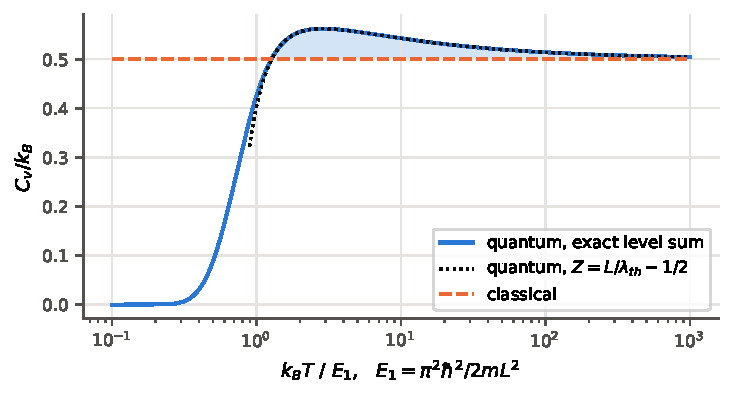
\includegraphics[width=0.7\textwidth]{fig_box_only.pdf}
\caption{Empty box: exact level sum (blue), Eq.~\eqref{eq:boxexcess} (dotted, drawn for $r<1.2$) and the classical $\kB/2$ (orange, dashed). The curve is the same for every $L$ when $T$ is measured in units of $E_1$.}
\label{fig:box}
\end{figure}

% =====================================================================
\section{The mechanism, and the numbers}
\label{sec:mechanism}

\subsection{Results}
Table~\ref{tab:anomaly} and Fig.~\ref{fig:cases} compare Eqs.~\eqref{eq:Cq} and \eqref{eq:Ccl}.

\begin{table}[h]
\centering
\caption{Quantum vs.\ classical heat capacity (\texttt{check\_formulas.py}, section 4). All temperatures are $\kB T$ in units of $\Eu$, on a grid up to 1. ``Window'' is where $\Cq>\Ccl$.}
\label{tab:anomaly}
\resizebox{\textwidth}{!}{%
\begin{tabular}{cccccccc}
\toprule
$\alpha L$ & $\max(\Cq-\Ccl)/\kB$ & at $\kB T$ & $\Cq/\kB$, $\Ccl/\kB$ there & window & $\Cq$ peak (at) & $\Ccl$ peak (at) & $\min(\Cq-\Ccl)/\kB$ (at)\\
\midrule
30 & none for $\kB T<1$ & -- & -- & -- & 2.00 (0.393) & 3.74 (0.412) & $-1.75$ (0.421)\\
100 & $+0.343$ & 0.210 & 2.427, 2.084 & $[0.176,0.239]$ & 3.56 (0.285) & 6.21 (0.344) & $-3.18$ (0.367)\\
400 & $+2.591$ & 0.184 & 5.091, 2.499 & $[0.129,0.223]$ & 6.05 (0.216) & 10.03 (0.283) & $-6.20$ (0.299)\\
1000 & $+4.802$ & 0.167 & 7.397, 2.595 & $[0.112,0.203]$ & 8.13 (0.185) & 13.13 (0.252) & $-9.10$ (0.263)\\
\bottomrule
\end{tabular}}
\end{table}

\begin{figure}[h]
\centering
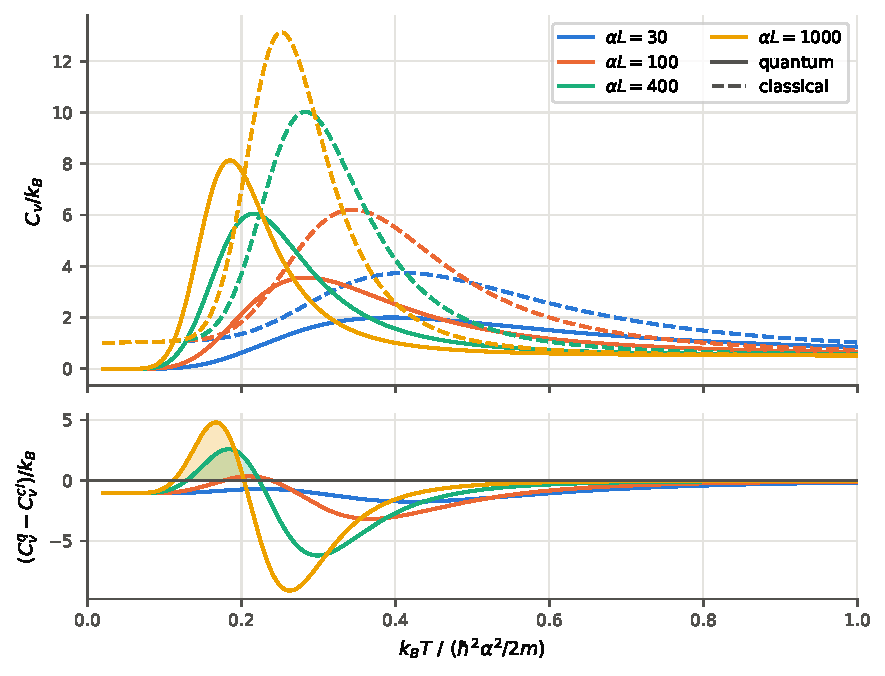
\includegraphics[width=0.8\textwidth]{fig_cv_cases.pdf}
\caption{$\Cq$ (solid) and $\Ccl$ (dashed) and their difference, for four box lengths. Shaded: $\Cq>\Ccl$.}
\label{fig:cases}
\end{figure}

\subsection{Heuristic 1: who desorbs first}
Both curves are dominated by one event, the particle leaving the well for the box (desorption). The transition sits roughly where the well and the box carry equal Boltzmann weight.
\begin{itemize}[itemsep=2pt]
\item \textbf{Quantum.} The well's weight is the single bound state, $e^{-\beta E_b}=e^{a/2}$; the box's is $L/\lth$. Equal weights give, with Eq.~\eqref{eq:helpers},
\begin{equation}
\frac{a_q}{2}=\ln\frac{L}{\lth}\quad\Longleftrightarrow\quad\frac{\Eu}{\kB T_q}=\ln\!\left(\alpha L\sqrt{\frac{\kB T_q}{4\pi\,(\Eu)}}\right).
\end{equation}
\item \textbf{Classical.} The well's weight is $I/\lth$. At low $T$ only the harmonic bottom matters, and Laplace's method gives $\alpha I\simeq e^{a}\sqrt{\pi/a}$, i.e.\ $I/\lth\simeq e^{a}\,\kB T/\hbar\omega_0$ with $\hbar\omega_0=\sqrt2\,\hbar^2\alpha^2/m$, the frequency of the bottom ($\frac12m\omega_0^2=\hbar^2\alpha^4/m$). The factor $\kB T/\hbar\omega_0$ is the classical oscillator's partition function: the entropy cost of being localized. Equal weights, $I=L$, give
\begin{equation}
a_{\rm cl}-\tfrac12\ln a_{\rm cl}=\ln\frac{\alpha L}{\sqrt\pi},\qquad \frac{\kB T_{\rm cl}}{\Eu}=\frac{2}{a_{\rm cl}}.
\end{equation}
\end{itemize}
In the relevant range the classical well holds more weight than the quantum one: their ratio is $[e^{a}/(\sqrt2a)]/e^{a/2}=e^{a/2}/(\sqrt2a)$, about 10 at $a=10$. The zero-point energy costs the quantum particle half the depth, more than localization costs the classical one. Hence $T_q<T_{\rm cl}$:
\begin{center}
\begin{tabular}{ccccc}
\toprule
$\alpha L$ & $\kB T_q$ estimate & $\Cq$ peak & $\kB T_{\rm cl}$ estimate & $\Ccl$ peak\\
\midrule
100 & 0.354 & 0.285 & 0.415 & 0.344\\
400 & 0.248 & 0.216 & 0.315 & 0.283\\
1000 & 0.206 & 0.185 & 0.273 & 0.252\\
\bottomrule
\end{tabular}
\end{center}
The estimates run 10--25\% high but reproduce the order $T_q<T_{\rm cl}$ and the growth of the gap with $\alpha L$.

\subsection{Heuristic 2: the peak heights}
Treat each system as two ``phases'', bound and gas, with occupation $p$ of the gas. A Schottky-type estimate gives a peak $C_v\approx\kB\,p(1-p)(\beta\Delta)^2\le\frac{\kB}{4}(\beta\Delta)^2$, where $\Delta$ is the energy gained on desorption. Quantum: from $-\hbar^2\alpha^2/2m$ to a gas with mean energy $\frac12\kB T$, so $\Delta_q=\Eu+\frac12\kB T$. Classical: from $-\hbar^2\alpha^2/m+\kB T$ (harmonic bottom) to $\frac12\kB T$, so $\Delta_{\rm cl}=\hbar^2\alpha^2/m-\frac12\kB T$. In units of $\Eu$, $\beta\Delta_q=\Eu/\kB T+\frac12$ and $\beta\Delta_{\rm cl}=2\,\Eu/\kB T-\frac12$. At the computed peak temperatures this gives $4.0$, $6.6$, $8.7$ (quantum) and $7.1$, $10.8$, $13.8$ (classical) for $\alpha L=100$, $400$, $1000$, against the computed $3.56$, $6.05$, $8.13$ and $6.21$, $10.03$, $13.13$, i.e.\ 5--15\% high. The classical peak is taller because its latent heat is about twice as large; the quantum peak comes first.

\subsection{The window}
Below both peaks, $\Cq\approx0$ (frozen in one state) while $\Ccl\approx\kB$ (vibrating in the bottom), so $\Cq<\Ccl$. As $T$ rises the quantum particle starts to desorb first. Its $\Cq$ rises steeply while the classical particle is still bound with $\Ccl\approx\kB$, and this is the window where $\Cq>\Ccl$. Then the classical desorption begins, with its larger latent heat, and the order reverses into a deficit (last column of Table~\ref{tab:anomaly}). The anomaly is a \emph{shift} of the peak to lower temperature, not a larger peak. A bigger box (larger $\alpha L$) means more states to desorb into, lower desorption temperatures, larger $\beta\Delta$ and sharper peaks, so the excess grows with $\alpha L$. The window first opens between $\alpha L=70$ and $80$: $\max(\Cq-\Ccl)=-0.04\kB$ at $\alpha L=70$ and $+0.10\kB$ at $\alpha L=80$.

% =====================================================================
\section{Homogeneous (scale-invariant) strokes}
\label{sec:stroke}

\subsection{Definition}
Deffner \emph{et al.}~\cite{deffner2014} call a driving scale-invariant when the Hamiltonian keeps the form of their Eq.~(3). For a dilation about $x=0$ (their $f=0$; their $U$ and $q$ are our $V$ and $x$),
\begin{equation}
H(\gamma)=\frac{p^2}{2m}+\frac{1}{\gamma^2}\,V_0\!\left(\frac{x}{\gamma}\right).
\label{eq:Hscale}
\end{equation}
A family $V(x;\mu)$ with control parameters $\mu$ admits such a stroke if there is a path $\mu(\gamma)$ with $\mu(1)=\mu_0$ and
\begin{equation}
V\big(x;\mu(\gamma)\big)=\frac{1}{\gamma^2}\,V\!\left(\frac{x}{\gamma};\mu_0\right)\qquad\text{for all }x\text{ and all }\gamma>0 .
\label{eq:scaleinv}
\end{equation}

\subsection{Each component, and their sum}
Write $V(x;\alpha,L)=V_{\rm PT}(x;\alpha)+V_{\rm box}(x;L)$ with $V_{\rm PT}=-\frac{\hbar^2}{2m}\alpha^2\frac{\lambda(\lambda-1)}{\cosh^2(\alpha x)}$ on $\mathbb R$ and $V_{\rm box}=0$ for $|x|<L/2$, $+\infty$ otherwise.
\begin{itemize}[itemsep=2pt]
\item \textbf{Well} (Table~I of Ref.~\cite{deffner2014}: $\alpha\to\alpha/\gamma$, $\lambda$ fixed):
\[
V_{\rm PT}\!\left(x;\tfrac{\alpha}{\gamma}\right)=-\frac{\hbar^2}{2m}\frac{\alpha^2}{\gamma^2}\frac{\lambda(\lambda-1)}{\cosh^2(\alpha x/\gamma)}=\frac{1}{\gamma^2}V_{\rm PT}\!\left(\frac{x}{\gamma};\alpha\right).
\]
The $\alpha^2$ in front supplies $\gamma^{-2}$; the $\alpha$ inside $\cosh$ supplies $x/\gamma$.
\item \textbf{Box} ($L\to\gamma L$; Table~I lists it as the $b\to\infty$ member of the power-law family): $|x|<\gamma L/2\iff|x/\gamma|<L/2$, and $\gamma^{-2}\cdot0=0$, $\gamma^{-2}\cdot\infty=\infty$, so $V_{\rm box}(x;\gamma L)=\gamma^{-2}V_{\rm box}(x/\gamma;L)$.
\item \textbf{Sum, same $\gamma$.} The map $U\mapsto\gamma^{-2}U(x/\gamma)$ is linear, so
\begin{equation}
V\!\left(x;\frac{\alpha}{\gamma},\gamma L\right)=\frac{1}{\gamma^2}\,V\!\left(\frac{x}{\gamma};\alpha,L\right).
\label{eq:sumscale}
\end{equation}
\item \textbf{Different factors fail.} With $\alpha\to\alpha/\gamma_1$ and $L\to\gamma_2L$, suppose the result were $c^{-2}V(x/c;\alpha,L)$. The walls force $c=\gamma_2$; the value at $x=0$ forces $\alpha^2/\gamma_1^2=\alpha^2/c^2$, i.e.\ $c=\gamma_1$. So $\gamma_1=\gamma_2$. Physically: the shape is set by $\alpha L$, and a scale-invariant stroke must keep it.
\end{itemize}

\subsection{All levels scale by the same factor}
Let $\psi_n$ solve the $\gamma=1$ problem with energy $E_n$ and $\psi_n(\pm L/2)=0$, and define $\psi_n^{(\gamma)}(x)=\gamma^{-1/2}\psi_n(x/\gamma)$ (the map of Ref.~\cite{deffner2014}, App.~A). Since $\dv[2]{x}\psi_n(x/\gamma)=\gamma^{-2}\psi_n''(x/\gamma)$ and by Eq.~\eqref{eq:sumscale},
\[
-\frac{\hbar^2}{2m}\dv[2]{\psi_n^{(\gamma)}}{x}+V\!\left(x;\tfrac\alpha\gamma,\gamma L\right)\psi_n^{(\gamma)}
=\frac{\gamma^{-1/2}}{\gamma^2}\left[-\frac{\hbar^2}{2m}\psi_n''+V(\,\cdot\,;\alpha,L)\,\psi_n\right]\!\left(\frac x\gamma\right)=\frac{E_n}{\gamma^2}\,\psi_n^{(\gamma)}(x),
\]
with the boundary condition moving with the walls and the norm preserved. The map is invertible, so
\begin{equation}
\boxed{\;E_n\!\left(\frac\alpha\gamma,\gamma L\right)=\frac{1}{\gamma^2}\,E_n(\alpha,L)\quad\text{for every }n.\;}
\label{eq:Escale}
\end{equation}
The exact equations agree: $\alpha L$ is unchanged and $\alpha\tanh(\alpha L/2)\to\alpha\tanh(\alpha L/2)/\gamma$, so the roots of Eqs.~\eqref{eq:quant}--\eqref{eq:bound} scale as $k_j\to k_j/\gamma$, $\kappa_b\to\kappa_b/\gamma$. Numerically, $\max_n|\gamma^2E_n(\text{after})-E_n(\text{before})|\le6\times10^{-17}$ for $\gamma=0.7,1.5,2$. This is \emph{homogeneous level scaling}, $E_n^{c}=qE_n^{h}$ with one $q=\gamma^{-2}$ for all $n$, in the language of Refs.~\cite{GK,LGK}.

\subsection{Partition functions and heat capacities}
Quantum: $Z_q(\beta;\frac\alpha\gamma,\gamma L)=\sum_ne^{-\beta E_n/\gamma^2}=Z_q(\beta/\gamma^2;\alpha,L)$. Classical: substitute $x=\gamma y$ and use Eq.~\eqref{eq:sumscale} and $\lth\propto\beta^{1/2}$,
\[
Z_{\rm cl}\!\left(\beta;\tfrac\alpha\gamma,\gamma L\right)=\frac{\gamma}{\lth(\beta)}\int e^{-(\beta/\gamma^2)V(y;\alpha,L)}\dd y=Z_{\rm cl}\!\left(\frac{\beta}{\gamma^2};\alpha,L\right).
\]
Since $\beta^2\partial_\beta^2$ is unchanged by $\beta\to\beta/\gamma^2$,
\begin{equation}
C_v(T;\gamma)=C_v(\gamma^2T;1)\qquad\text{for both }\Cq\text{ and }\Ccl,
\label{eq:Cvscale}
\end{equation}
checked numerically to $2\times10^{-12}\kB$ (Fig.~\ref{fig:stroke}). The stroke slides every feature, the anomaly window included, from $T^*$ to $T^*/\gamma^2$, without changing its shape or height. This is consistent with Sec.~\ref{sec:model}: the stroke keeps $\alpha L$, and $\kB T/(\Eu)$ is the same at $(T,\alpha/\gamma)$ as at $(\gamma^2T,\alpha)$.

\begin{figure}[h]
\centering
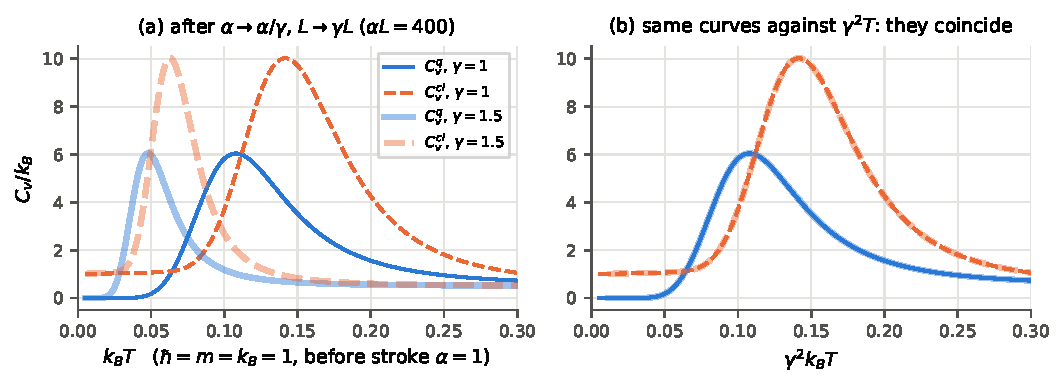
\includegraphics[width=\textwidth]{fig_stroke.pdf}
\caption{A scale-invariant stroke, $\alpha\to\alpha/\gamma$, $L\to\gamma L$ with $\gamma=1.5$ ($\alpha L=400$ kept). (a) The curves move to lower $T$. (b) Against $\gamma^2T$ they coincide with the $\gamma=1$ curves.}
\label{fig:stroke}
\end{figure}

\subsection{Why this matters for the engine: \texorpdfstring{$Q$}{Q} and \texorpdfstring{$W$}{W} from \texorpdfstring{$C_v$}{Cv}}
This follows Levy and Gelbwaser-Klimovsky~\cite{LGK}, Eqs.~(4.15)--(4.18), in their notation: hot-stroke Hamiltonian $H_h$, cold-stroke Hamiltonian $H_c$, $E_n^{c}=qE_n^{h}$ (here $q=\gamma^{-2}$ for an expansion $\gamma>1$). The Otto cycle is A $\to$ B (adiabatic $H_h\to H_c$) $\to$ C (cold bath $T_c$) $\to$ D (adiabatic $H_c\to H_h$) $\to$ A (hot bath $T_h$).
\begin{enumerate}[itemsep=2pt]
\item A is thermal at $T_h$ for $H_h$: $p_n^A\propto e^{-E_n^h/\kB T_h}$.
\item A slow (quantum-adiabatic) stroke keeps the populations, and homogeneous scaling keeps the level order, so no level crossings occur.
\item C is thermal at $T_c$ for $H_c$: $p_n^C\propto e^{-E_n^c/\kB T_c}=e^{-E_n^h/\kB(T_c/q)}$. After the stroke C $\to$ D the populations are unchanged, so D is \emph{thermal for $H_h$ at $T_c/q$}. Likewise B is thermal for $H_c$ at $qT_h$.
\item Hence, with $U_h(T)$ the thermal energy of $H_h$ and $U_c(T)=qU_h(T/q)$,
\begin{align}
Q_h&=\expval{H_h}_A-\expval{H_h}_D=U_h(T_h)-U_h(T_c/q)=\int_{T_c/q}^{T_h}C_v\,\dd T,\\
Q_c&=\expval{H_c}_C-\expval{H_c}_B=q\big[U_h(T_c/q)-U_h(T_h)\big]=-q\int_{T_c/q}^{T_h}C_v\,\dd T,\\
W&=-(Q_h+Q_c)=(q-1)\int_{T_c/q}^{T_h}C_v\,\dd T,\qquad \eta=-\frac{W}{Q_h}=1-q,
\label{eq:Wcv}
\end{align}
where $C_v$ is the heat capacity of $H_h$. An engine ($W<0$) needs $T_c/T_h<q<1$.
\end{enumerate}
Gelbwaser-Klimovsky \emph{et al.}~\cite{GK}, Eq.~(2), state the same result with their $q$ equal to our $1/q$, and note that it also follows from a fully classical treatment with the classical $C_v$. \emph{Heuristic for the classical side:} in a slow 1D stroke the action $J=\oint p\,\dd x$ is an adiabatic invariant (Landau and Lifshitz, \emph{Mechanics}~\cite{LLmech}, \S49). Under Eq.~\eqref{eq:sumscale} an orbit maps as $x\to\gamma x$, $p\to p/\gamma$, which keeps $J$ and multiplies $H$ by $\gamma^{-2}$. So $E(J)\to E(J)/\gamma^2$ for every orbit, and a canonical distribution again maps to a canonical one at a scaled temperature.

\paragraph{Consequence.} The efficiency is the same for both, $\eta=1-q$, but by Eq.~\eqref{eq:Wcv} the work and heat are set by $\int C_v\,\dd T$ alone. If $[T_c/q,T_h]$ lies inside a window where $\Cq>\Ccl$, the quantum engine extracts more work at equal efficiency. The windows are narrow: at $\alpha L=1000$, $[0.112,0.203]\,(\Eu)$, a ratio of 1.8, so $T_h/(T_c/q)\le1.8$.

% =====================================================================
\section{What to double-check before presenting}
\label{sec:verify}
\begin{enumerate}[itemsep=2pt]
\item \textbf{Confirmed from the PDFs in \texttt{docs/refs}:} Deffner \emph{et al.}~\cite{deffner2014} Eq.~(3), Table~I (modified P\"oschl--Teller row, citing Fl\"ugge; power-law row including the infinite well); Levy and Gelbwaser-Klimovsky~\cite{LGK} Eqs.~(4.15)--(4.18) and Fig.~4.3 (box $\Cq>\Ccl$); Gelbwaser-Klimovsky \emph{et al.}~\cite{GK} Eq.~(2) and the definition of homogeneous scaling.
\item \textbf{Quoted from memory, so check the numbers in a library copy:} Landau--Lifshitz QM \S23 Problem~4 (levels of $-U_0/\cosh^2\alpha x$) and \S25 Problem~4 (its transmission coefficient); Landau--Lifshitz \emph{Mechanics} \S49; Fl\"ugge's problem title; Pathria--Beale \S\S3.5--3.7 (3rd ed.); Gradshteyn--Ryzhik 3.466.1 (7th ed.); DLMF \S1.8(iv), \S5.12, Ch.~7; the volume and page of Lekner~\cite{lekner} and Levinson~\cite{levinson}. The \emph{content} of each is also derived here, so nothing depends on the numbering.
\item \textbf{Approximations:} terms of order $e^{-\alpha L}$ (Sec.~\ref{sec:model}) and the Poisson remainder $R$ (exponentially small for $L\gtrsim\lth$) are dropped. Both are checked numerically against exact level sums.
\item \textbf{Heuristics are heuristics:} the equal-weight temperatures run 10--25\% high and the peak-height estimate 5--15\% high. They explain the ordering, not the exact numbers.
\item \textbf{Hard walls:} because of the wall term, $\int_0^\infty(\Cq-\Ccl)\,\dd T$ diverges here, so the zero-point sum rule that holds for smooth confining potentials does not apply.
\end{enumerate}

% =====================================================================
\appendix
\section{Direct check of \texorpdfstring{$\psi_k$}{psi\_k}}
\label{app:check}
With $u=\tanh(\alpha x)$, $u'=\alpha(1-u^2)$:
\begin{align*}
\psi_k&=(\alpha u-ik)e^{ikx},\\
\psi_k'&=\big[\alpha^2(1-u^2)+ik\alpha u+k^2\big]e^{ikx},\\
\psi_k''&=\big[-2\alpha^3u(1-u^2)+2ik\alpha^2(1-u^2)-k^2\alpha u+ik^3\big]e^{ikx}.
\end{align*}
The Schr\"odinger equation is $-\psi''-2\alpha^2(1-u^2)\psi=k^2\psi$, since $\frac{2m}{\hbar^2}V=-2\alpha^2/\cosh^2(\alpha x)=-2\alpha^2(1-u^2)$ and $E=\hbar^2k^2/2m$. Substituting,
\[
-\psi_k''-2\alpha^2(1-u^2)\psi_k=\big[k^2\alpha u-ik^3\big]e^{ikx}=k^2(\alpha u-ik)e^{ikx}=k^2\psi_k .\qquad\checkmark
\]

\section{The Gaussian--Lorentzian integral}
\label{app:gaussint}
For $c>0$ let $\mathcal F(b)=\int_0^\infty e^{-bk^2}/(k^2+c^2)\,\dd k$. Then
\[
\mathcal F'(b)-c^2\mathcal F(b)=-\int_0^\infty e^{-bk^2}\dd k=-\frac12\sqrt{\frac{\pi}{b}},
\qquad\text{so}\qquad
\dv{b}\big(e^{-bc^2}\mathcal F\big)=-\frac12\sqrt{\frac\pi b}\,e^{-bc^2}.
\]
Integrate from $b$ to $\infty$, where $e^{-bc^2}\mathcal F\to0$, and substitute $s=u^2/c^2$:
\[
\mathcal F(b)=e^{bc^2}\int_b^\infty\frac12\sqrt{\frac\pi s}\,e^{-sc^2}\dd s=\frac{\sqrt\pi}{c}\,e^{bc^2}\int_{c\sqrt b}^\infty e^{-u^2}\dd u=\frac{\pi}{2c}\,e^{bc^2}\erfc\!\left(c\sqrt b\right),
\]
which is Gradshteyn--Ryzhik 3.466.1~\cite{GR}.

\section{The classical well integrals}
\label{app:classint}
$\alpha J_1=\int_{-1}^1e^{a(1-t^2)}\dd t=2e^a\int_0^1e^{-at^2}\dd t$, and with $u=t\sqrt a$, $\int_0^1e^{-at^2}\dd t=\frac{1}{\sqrt a}\int_0^{\sqrt a}e^{-u^2}\dd u=\frac{\sqrt\pi}{2\sqrt a}\erf\sqrt a$. So $\alpha J_1=\sqrt\pi\,e^a\erf\sqrt a/\sqrt a$. Differentiating, with $\dd\erf\sqrt a/\dd a=\frac{2}{\sqrt\pi}e^{-a}\frac{1}{2\sqrt a}=e^{-a}/\sqrt{\pi a}$,
\[
\alpha J_2=\dv{(\alpha J_1)}{a}=\sqrt\pi\,e^a\erf\sqrt a\left(a^{-1/2}-\tfrac12a^{-3/2}\right)+\frac1a=\alpha J_1\left(1-\frac1{2a}\right)+\frac1a .
\]
Also $\dd(\alpha I)/\dd a=\alpha J_1$, consistent with Eq.~\eqref{eq:I}: differentiating the series term by term gives $\sum_\ell 2^\ell a^{\ell-1}/(2\ell-1)!!$, which is the series of $2e^a\int_0^1e^{-at^2}\dd t$.

% =====================================================================
\begin{thebibliography}{99}
\bibitem{deffner2014} S. Deffner, C. Jarzynski, and A. del Campo, ``Classical and quantum shortcuts to adiabaticity for scale-invariant driving,'' Phys.\ Rev.\ X \textbf{4}, 021013 (2014).
\bibitem{flugge} S. Fl\"ugge, \emph{Practical Quantum Mechanics} (Springer, Berlin, 1971), problem ``Modified P\"oschl--Teller potential hole''.
\bibitem{poschlteller} G. P\"oschl and E. Teller, ``Bemerkungen zur Quantenmechanik des anharmonischen Oszillators,'' Z.\ Phys.\ \textbf{83}, 143 (1933).
\bibitem{LL} L. D. Landau and E. M. Lifshitz, \emph{Quantum Mechanics (Non-relativistic Theory)}, 3rd ed.\ (Pergamon, Oxford, 1977), \S23 Problem~4 and \S25 Problem~4.
\bibitem{LLmech} L. D. Landau and E. M. Lifshitz, \emph{Mechanics}, 3rd ed.\ (Pergamon, Oxford, 1976), \S49.
\bibitem{lekner} J. Lekner, ``Reflectionless eigenstates of the sech$^2$ potential,'' Am.\ J.\ Phys.\ \textbf{75}, 1151 (2007).
\bibitem{CKS} F. Cooper, A. Khare, and U. Sukhatme, ``Supersymmetry and quantum mechanics,'' Phys.\ Rep.\ \textbf{251}, 267 (1995).
\bibitem{levinson} N. Levinson, ``On the uniqueness of the potential in a Schr\"odinger equation for a given asymptotic phase,'' Kgl.\ Danske Vid.\ Selsk.\ Mat.-fys.\ Medd.\ \textbf{25}, no.~9 (1949).
\bibitem{pathria} R. K. Pathria and P. D. Beale, \emph{Statistical Mechanics}, 3rd ed.\ (Elsevier, Oxford, 2011).
\bibitem{dlmf} F. W. J. Olver \emph{et al.} (eds.), \emph{NIST Digital Library of Mathematical Functions}, \url{https://dlmf.nist.gov}.
\bibitem{BU} E. Beth and G. E. Uhlenbeck, ``The quantum theory of the non-ideal gas. II. Behaviour at low temperatures,'' Physica \textbf{4}, 915 (1937).
\bibitem{DMB} R. Dashen, S.-K. Ma, and H. J. Bernstein, ``S-matrix formulation of statistical mechanics,'' Phys.\ Rev.\ \textbf{187}, 345 (1969).
\bibitem{GR} I. S. Gradshteyn and I. M. Ryzhik, \emph{Table of Integrals, Series, and Products}, 7th ed.\ (Academic Press, 2007).
\bibitem{LGK} A. Levy and D. Gelbwaser-Klimovsky, ``Quantum features and signatures of quantum thermal machines,'' in \emph{Thermodynamics in the Quantum Regime}, F. Binder, L. A. Correa, C. Gogolin, J. Anders, and G. Adesso (eds.), Fundamental Theories of Physics \textbf{195}, 87 (Springer, 2018).
\bibitem{GK} D. Gelbwaser-Klimovsky, A. Bylinskii, D. Gangloff, R. Islam, A. Aspuru-Guzik, and V. Vuleti\'c, ``Single-atom heat machines enabled by energy quantization,'' Phys.\ Rev.\ Lett.\ \textbf{120}, 170601 (2018).
\end{thebibliography}

\end{document}
